%\documentclass{article}
\documentclass[class=minimal,border=4pt]{standalone}
\usepackage{tikz}
\usetikzlibrary{patterns}
\newcommand\actfill{1.0}
\newcommand\actcol{yellow}
\newcommand\tikscale{0.32}
\newcommand{\smiley}{\tikz[baseline=-0.75ex,black]{
\filldraw[fill=orange!10] circle (2mm);
\node[fill,circle,inner sep=0.5pt] (left eye) at (135:0.8mm) {};
\node[fill,circle,inner sep=0.5pt] (right eye) at (45:0.8mm) {};
\draw[-] (-145:0.9mm) arc (-120:-60:1.5mm);
}
}
\newcommand{\frownie}{\tikz[baseline=-0.75ex,black]{
\filldraw[fill=red!20] circle (2mm);
\node[fill,circle,inner sep=0.5pt] (left eye) at (135:0.8mm) {};
\node[fill,circle,inner sep=0.5pt] (right eye) at (45:0.8mm) {};
\draw[-] (-145:0.9mm) arc (120:60:1.5mm);
}
}

\pgfdeclarepatternformonly{dark lines}{\pgfqpoint{-1pt}{-1pt}}{\pgfqpoint{12pt}{12pt}}{\pgfqpoint{12pt}{12pt}}%
{
  \pgfsetlinewidth{3pt}
  \pgfpathmoveto{\pgfqpoint{0pt}{0pt}}
  \pgfpathlineto{\pgfqpoint{12pt}{12pt}}
  \pgfusepath{stroke}
}

   
\begin{document}
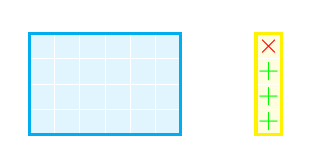
\begin{tikzpicture}[
fill opacity=.6,draw opacity=1,scale=\tikscale,
emptynode/.style={square}
]
%\fill[opacity=\actfill,\actcol] (1,8) rectangle (3,7);
%\fill[opacity=\actfill,\actcol] (3,7) rectangle (5,6);
%\fill[opacity=\actfill,\actcol] (0,5) rectangle (1,4);
%\fill[opacity=\actfill,\actcol] (2,5) rectangle (6,4);
%\fill[opacity=\actfill,\actcol] (0,3) rectangle (2,2);
%\fill[opacity=\actfill,\actcol] (3,2) rectangle (4,1);
%\fill[opacity=\actfill,\actcol] (5,1) rectangle (6,0);
%\fill[opacity=\actfill,\actcol] (0,0) rectangle (6,8);
\fill[fill=cyan!20, very thick] (0,0) rectangle (6,4);
\draw[ystep=1cm,xstep=1cm,white,very thin] (0,0) grid (6,4);
\draw[color=cyan, very thick] (0,0) rectangle (6,4);
\fill[fill=yellow!20, very thick] (9,0) rectangle (10,4);
\draw[ystep=1cm,xstep=1cm,white,very thin] (9,0) grid (10,4);
\draw[color=yellow, very thick] (9,0) rectangle (10,4);
\foreach \i in {0,1,2}
{
\node at (9.5,\i+0.5) [fill opacity=1,color=green] {$+$};
}
\foreach \i in {3}
{
\node at (9.5,\i+0.5) [fill opacity=1,color=red] {$\times$};
}

%\draw[ystep=1cm,xstep=1cm,gray,very thin] (9,0) grid (12,8);

%\draw[ultra thick,-] (3,0) -- (3,8);
%\draw[thin,-] (0,1) -- (6,1);
%\draw[thin,-] (0,2) -- (6,2);
%\draw[thin,-] (0,3) -- (6,3);
%\draw[thin,-] (0,4) -- (6,4);
%\draw[thin,-] (0,5) -- (6,5);
%\draw[thin,-] (0,6) -- (6,6);
%\draw[thin,-] (0,7) -- (6,7);
%\draw[magenta,ultra thick,->] plot[smooth,tension=1] coordinates {(1.25,7.5) (1.4,0.5) (4.55,7.5) (4.7,0.5)};
\end{tikzpicture}
\end{document}

